\documentclass[runningheads]{llncs}

\usepackage[T1]{fontenc}
\usepackage{graphicx}
\usepackage{listings}
\usepackage{xcolor}
\usepackage{pdfpages}
\usepackage{hyperref}

\lstset{
    language=HTML,
    basicstyle=\ttfamily\small,
    keywordstyle=\color{blue},
    stringstyle=\color{orange},
    commentstyle=\color{gray},
    breaklines=true,
    frame=single,
    numbers=left,
    numberstyle=\tiny\color{gray},
    showstringspaces=false,
}

\begin{document}

\title{Módulo 1: Los Pookies}

\author{Allamand Francisco \and
Mateo Notti Echave \and
Facundo Dip \and
Pedro Elizalde}



\institute{Universidad Nacional de Cuyo\\
\email{franallamand05@gmail.com}}

\maketitle

\begin{abstract}
En este trabajo se presentan los conocimientos adquiridos durante el Módulo 1, enfocados en el uso de lenguajes de marcado y herramientas digitales orientadas al desarrollo académico y profesional. Se abordan conceptos fundamentales de HTML, Markdown y LaTeX, junto con su aplicación práctica en la estructuración de documentos y contenidos web. Además, se incorporan recursos de referencia y la integración de documentación personal como parte del aprendizaje.
\end{abstract}

\section{Introducción}
A lo largo de este módulo se produjo una transición desde el uso básico de herramientas digitales hacia la adopción de metodologías más estructuradas y profesionales. El aprendizaje de lenguajes de marcado como HTML, Markdown y LaTeX permitió comprender cómo organizar información de manera clara, reutilizable y estandarizada \cite{github, markdown, latex}.

Este informe tiene como objetivo mostrar la aplicación concreta de estos lenguajes mediante ejemplos prácticos, destacando su utilidad tanto en el desarrollo web como en la producción de documentos técnicos. Asimismo, se evidencia la importancia del trabajo colaborativo y el uso de herramientas como GitHub en entornos académicos vinculados a la ingeniería \cite{git}.

\section{Uso avanzado de HTML}

\subsection{Ejemplo completo}
\begin{lstlisting}[language=HTML, caption=Ejemplo completo de HTML]
<!DOCTYPE html>
<html lang="es">
<head>
    <meta charset="UTF-8">
    <title>Ejemplo Completo</title>
</head>
<body>

<h1>Bienvenido</h1>
<p><b>Texto en negrita</b> y <i>texto en italica</i></p>

<hr>

<h2>Lista</h2>
<ul>
<li>Elemento 1</li>
<li>Elemento 2</li>
</ul>

<h2>Tabla</h2>
<table border="1">
<tr>
<th>Nombre</th>
<th>Edad</th>
</tr>
<tr>
<td>Juan</td>
<td>20</td>
</tr>
</table>

<h2>Enlaces</h2>
<a href="https://www.google.com">Ir a Google</a>

<h2>Imagen</h2>
<img src="imagen.jpg" alt="Ejemplo">

</body>
</html>
\end{lstlisting}

\subsection{Segundo ejemplo HTML}
\begin{lstlisting}[language=HTML, caption=Segundo ejemplo HTML]
<!DOCTYPE html>
<html>
<body>

<h1>Pagina simple</h1>

<p>Ir a una seccion interna:</p>
<a href="#seccion">Seccion</a>

<h2 id="seccion">Seccion interna</h2>
<p>Contenido de la seccion.</p>

</body>
</html>
\end{lstlisting}

\section{Lenguajes de Marcado}

\subsection{Markdown}
\begin{lstlisting}[caption=Ejemplo Markdown]
# Titulo
## Subtitulo

Texto en **negrita** y *italica*

- Item 1
- Item 2

[Link](https://github.com)
\end{lstlisting}

\subsection{LaTeX}
\begin{lstlisting}[language=TeX, caption=Ejemplo LaTeX]
\section{Seccion}
Texto con cita \cite{latex}.

\begin{itemize}
\item Punto 1
\item Punto 2
\end{itemize}
\end{lstlisting}

\section{Cheatsheets}

Para la correcta implementación de los lenguajes de marcado y el uso de las herramientas del módulo, se consultaron las siguientes guías rápidas y documentación oficial:

\begin{itemize}
\item \href{https://www.markdownguide.org/cheat-sheet/}{Markdown Cheat Sheet} \cite{markdown}
\item \href{https://www.w3schools.com}{HTML Reference} \cite{html}
\item \href{https://www.overleaf.com/learn}{LaTeX Guide} \cite{latex}
\item \href{https://education.github.com}{GitHub Guide} \cite{git}
\end{itemize}

\section{Conclusión}
El desarrollo de este módulo permitió incorporar herramientas fundamentales para la formación en ingeniería, especialmente en lo relacionado con la organización y presentación de información técnica. La utilización de lenguajes de marcado representa un cambio significativo respecto a métodos tradicionales, ya que favorece la claridad estructural, la reutilización de contenido y la adaptación a distintos formatos.

En el ámbito profesional, estas habilidades resultan especialmente valiosas para la elaboración de informes técnicos, documentación de proyectos y comunicación efectiva dentro de equipos de trabajo. Asimismo, el uso de plataformas como GitHub introduce prácticas propias del entorno laboral, como el control de versiones y el trabajo colaborativo distribuido.

A futuro, el dominio de estas herramientas permitirá abordar proyectos de mayor complejidad, integrando desarrollo web, documentación técnica y gestión de información en un mismo flujo de trabajo. Esto resulta particularmente relevante en ingeniería, donde la precisión, la organización y la capacidad de adaptación tecnológica son competencias clave.

\section{Anexos}

% PDFs de CV
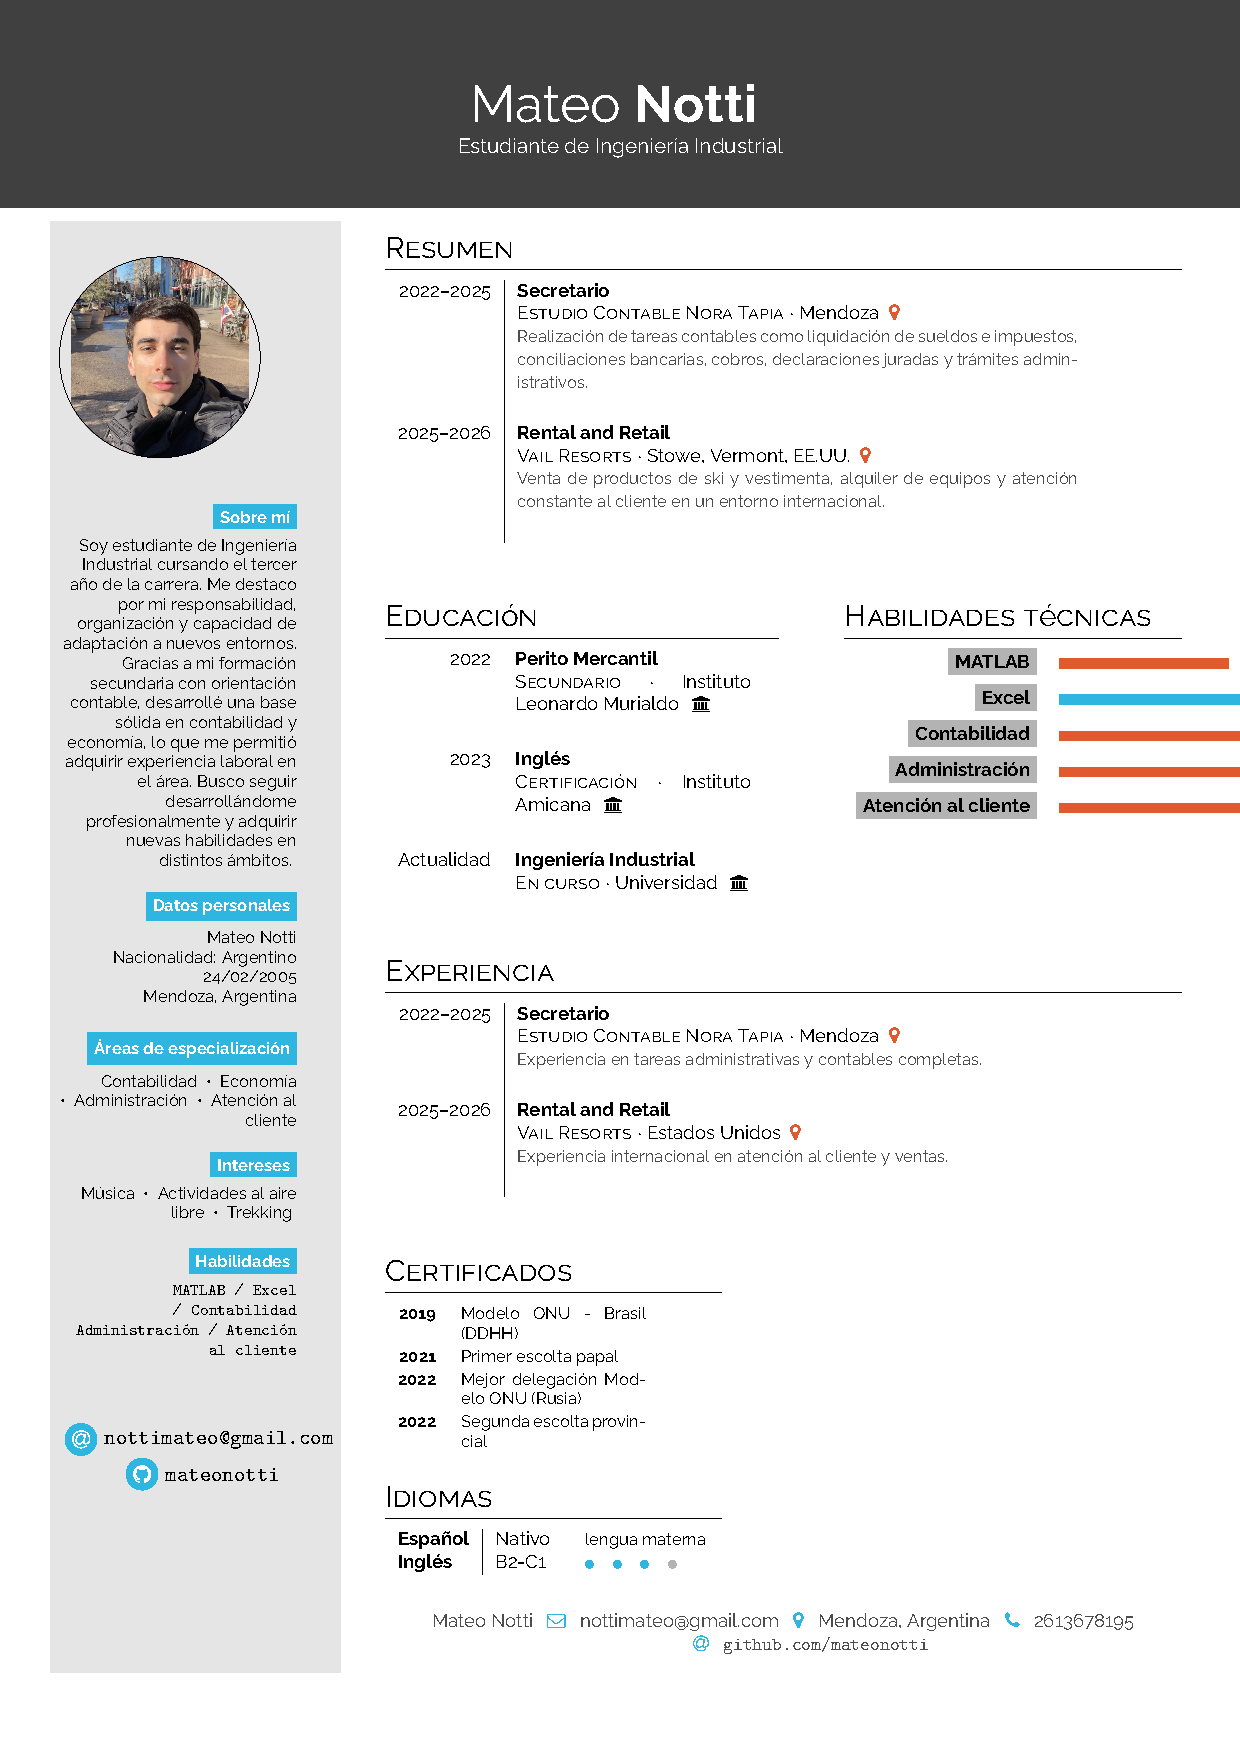
\includepdf[pages=-, pagecommand={\thispagestyle{plain}}]{mateonotticv.pdf}

\bibliographystyle{splncs04}
\bibliography{bibliografia}

\end{document}